\chapter{Blind GNSS Search of Extraterrestrial EUV Sources}

In the previous chapter we saw that an algorithm for detecting the location of an EUV source (in this case, the Sun) is possible with a first, brute force approach. Here, several optimizations are presented for the algorithm to reduce its computational complexity. Some of which are built on top of each other.

\section{Decreasing the range of the search}

As we saw in the previous chapter, to increase the precision of the algorithm, the \textit{step} with which we iterate over the possible angles (right ascension and declination) is reduced. This causes more possible Suns to be considered. For example, with a step of one degree, we consider all possible right ascensions [0,360] and declinations [-90,90] which is  $360*180 = 64800$ Suns, minus the $2*360 - 2 = 718$ right ascensions we don't consider because as we have seen right ascensions for declinations of -90 and 90 are the same location.

We want to have the highest precision possible without having to consider all $64800 - 718 = 64082$ possibilities by progressively reducing the search range. 

\subsection{Pseudocode}

This first optimization works as follows: the entire possible range is considered with a large starting step (e.g 60). Once the best Sun is found within this range, the precision is increased (the step is decreased) and the search range is reduced. This way the precision is increased but the number of considered possibilities remains similar each iteration of the algorithm. The following is the pseudocode\footnote{The code for the special cases of -90 and 90 degree declinations is not included for more readability. It is included in the implantation, in the following section.} for the algorithm using this optimization:

\begin{algorithm}
	\caption{Search range decrease}\label{searchRangeDecrease}
	\begin{algorithmic}[1]
		\Procedure{main}{}
		\State $\textit{epoch} \gets \text{findSpikeInData()}$ 
		\State $\text{filterDataByEpoch(\textit{epoch})}$
		\State $bestSun \gets nil$
		\State $range \gets \text{defaultRange()}$ 
		\For {$step = initStep; step >= min; step\ /= 2$}
		\For {$ra = r.lowerRa;\ ra <= r.upperRa;\ ra += step$}
		\For {$dec = r.lowerDec;\ dec <= r.upperDec;\ dec += step$}
		\State $currentSun \gets computeCorrelationPossibleSun(ra, dec)$
		\If {$currentSun.correlation > bestSun.correlation$} 
		\State $bestSun \gets currentSun$
		\State $range \gets \text{newRange(\textit{bestSun, step})}$ 
		\EndIf
		\EndFor
		\EndFor
		\EndFor
		\\
		\Return $bestSun$
		\EndProcedure
	\end{algorithmic}
\end{algorithm}

Later in this section a study on the optimal parameters (starting value and decreasing rate) for this method is done. 

\subsection{Implementation}

\subsection{Results}

\clearpage

\section{Hill Climbing}

Using the previous optimization we can see a plot of all the possibilities the algorithm considers:

\begin{figure}[!htb]
	\begin{centering}
		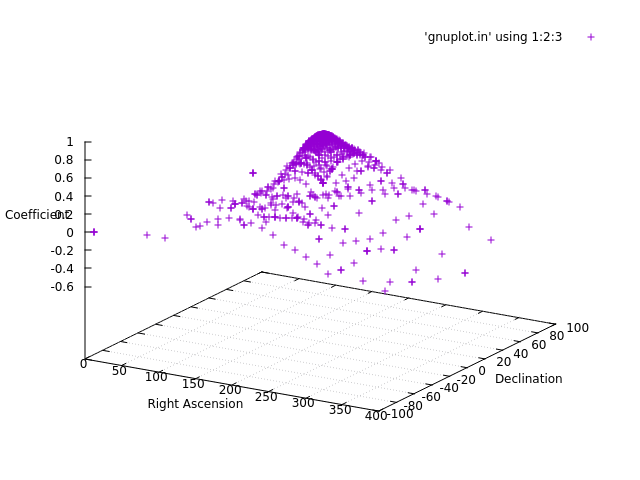
\includegraphics[width=0.6\linewidth]{images/ch6/hillClimbing/resultsAll.png}
		\caption{All visited candidates of the solution space}
		\label{fig:solutionSpace}
	\end{centering}
\end{figure}

As we can see in the previous figure, there appears to be a "hill" (our solution) so an attempt to solve the problem using a \textit{Hill Climbing} approach was also considered.

\begin{figure}[!htb]
	\begin{subfigure}[b]{0.5\textwidth}
		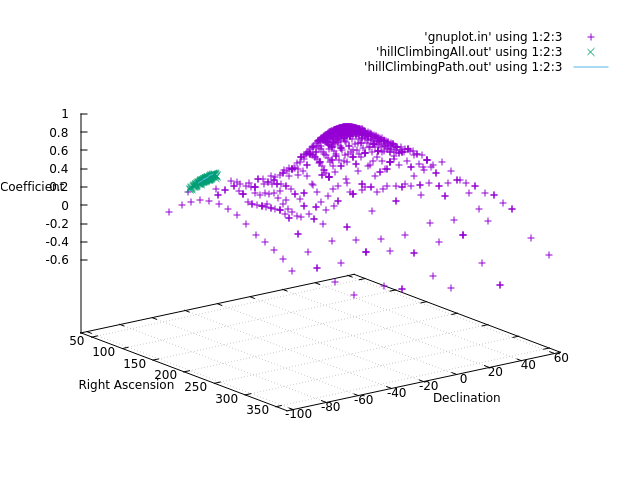
\includegraphics[width=\linewidth]{images/ch6/hillClimbing/resultsPathBad.png}
		\caption{Start: ra=100º, dec=-60º}
	\end{subfigure}
	\hfill
	\begin{subfigure}[b]{0.5\textwidth}
		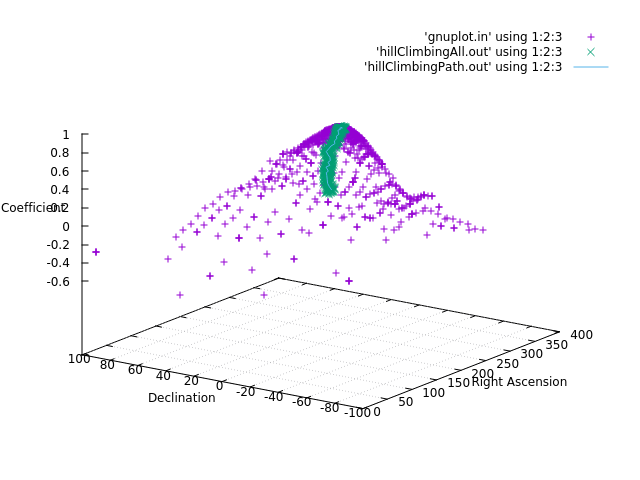
\includegraphics[width=\linewidth]{images/ch6/hillClimbing/resultsPathGood.png}
		\caption{Start: ra=160º, dec=-20º}
	\end{subfigure}
	\caption{Paths taken by the Hill Climbing algorithm}
	\label{fig:hillClimbingPaths}
\end{figure}

If we take ra 160, dec -20, good:


If we take 100, -60:


because of this blab ladasda as another possibility would be to use Simulated Annealing so that the algorithm doesn't stop in local hills.


\clearpage
\section{OpenMP?}


\section{Discarding the Sun hemisphere}

So far the algorithm has been studied for the case of the Sun, as it is a source that should be detected more easily than far-away stars. 

The main idea is that the algorithm should detect extraterrestrial EUV sources (if possible) other than the Sun. it follows that it should, before any other computations, discard the Sun hemisphere based on the current Sun location. The greater impact of the Sun's radiation due to its proximity would blind the algorithm from detecting sources that may be having an effect on that hemisphere because of the noise.